\chapter{Old stuff}
\section{Shortest Path Problems}
\subsection{Introduction}
% Something about the importance of this problem family
\subsection{All pairs shortest path}
Here we see the power of exchanging the semiring for the first time. In this section we will use the tropical semiring $(\R \cup \{\infty\}, \min, +)$ and its induced matrix operations. But first we have to state the problem:
\begin{problem}[All pairs shortest path] 
    Given a directed weighted graph $G = (V, E)$ with $|V| = n$ and $|E| = m$ and its adjacency matrix $A$. Compute the length of the shortest path between every pair of nodes.
\end{problem}

\begin{lemma}
    Let $A \in \R^{n \times n}$ be an adjacency matrix. Then $(A^k)_{ij}$ holds the length of the shortest path with $k+1$ nodes between $v_i$ and $v_j$ for all $k \in \N$. 
\end{lemma}
\begin{proof}
    Let $D_k \in \R^{n \times n}$ ba a matrix such that $(D_k)_{ij}$ holds the length of the shortest path with $k+1$ nodes between $v_i$ and $v_j$. Thus we need to show that $A^k = D_k$ for all $k \in \N$ which we will do by induction. Namely, we need to show that (I) $D_0 = \imat_n$ and (II) $D_{k+1} = D_k \odot A$
    \begin{enumerate}
        \item[(I)] ...
        \item[(II)] ...
    \end{enumerate}
\end{proof}

\begin{lemma}
    Let $A \in \R^{n \times n}$ be an adjacency matrix of a directed weighted graph $G$. Then $G$ has no negative cycle $\Leftrightarrow$ 
    $$\sum_{k=0}^{n-1+q} A^k = \sum_{k=0}^{n-1} A^k \quad\forall q \in \N$$
\end{lemma}

\begin{corollary}
    A direct conclusion of the last lemma is that
    $$A^* = \sum_{k=0}^{\infty}A^k = \sum_{k=0}^{n-1}A^k$$
\end{corollary}

And $A^*$ solves our problem.

\subsubsection{Optimisiation in shortest path}
As we allready stated, shortest path only exist iff no negative cycles are present in the graph. This also means that if loop edges exist, their weight must be positive. Thus no shortest path will pass through these loops, because any path passing through these edges can be shortened by just removing this edge. So even if loops exist in the graph, they can be ignored for the shortest path calculations. We will modify the graph such that every vertex has a loop with weight 0, resulting in a new adjacency matrix $\tilde A$:
$$\tilde A_{ij} = \begin{cases}
    0  &\textrm{if}\quad i = j\\
    A_{ij} &\textrm{else}
\end{cases}$$
And it will hold that
$$A^* = \sum_{k=0}^{n-1}\tilde A^k$$

Using the next lemma we can simplify our computation:
\begin{lemma}
    Let $(S, \oplus, \odot, 0, 1)$ be an semiring such that $\oplus$ is idempotent and $(S^{n \times n}, \boxplus, \boxdot, \zeromat, \imat)$ the semiring of matrix operations induced by $S$. Let $M, A \in S^{n \times n}$ such that $\forall i \in [n]: A_{ii} = 1$. Than it holds that:
    $$(M \boxdot A) \boxplus M = M \boxdot A$$ 
\end{lemma}
\begin{proof}
    \begin{align*}
        ((M\boxdot A) \boxplus M)_{ij} &= (M\boxdot A)_{ij} \oplus M_{ij} = (M\boxdot A)_{ij} \oplus( M_{ij} \odot \underbrace{A_{jj}}_1)\\
        &= (M_{i1} \odot A_{1j}) \oplus \dots \oplus (M_{ij} \odot A_{jj}) \oplus \dots \oplus (M_{in} \odot A_{nj}) \oplus (M_{ij} \odot A_{jj})\\
        &= (M_{i1} \odot A_{1j}) \oplus \dots \oplus (M_{in} \odot A_{nj}) \oplus \underbrace{(M_{ij} \odot A_{jj}) \oplus (M_{ij} \odot A_{jj})}_{(M_{ij} \odot A_{jj})}\\
        &= (M_{i1} \odot A_{1j}) \oplus \dots \oplus (M_{ij} \odot A_{jj}) \oplus \dots \oplus (M_{in} \odot A_{nj}) = (M \boxdot A)_{ij}
    \end{align*}
\end{proof}
Because $\tilde A$ has the neutral element of $\odot = +$ on its diagonal and $\oplus = \min$ is idempotent we can apply this lemma, resulting in $\tilde A^{k+1} \boxplus \tilde A^k = \tilde A^{k+1}$ and thus the sum for computing $A^*$ collapses to the simple expression:
$$A^* = \tilde A^{n-1}$$

This result could also be achieved by looking at the problem from the graph theory perspective. $A^*_{ij}$ holds the length of shortest path between $v_i$ and $v_j$ of any number of edges less than $n$. But if every vertex has a loop with weight 0, every such path can be extended to a path with $n-1$ edges while preserving its length. So every shortest path with less than $n-1$ edges is a shortest path with $n-1$ edges und thus $A^* = \tilde A^{n-1}$.
% Schnelle Matruxmult: https://www.sciencedirect.com/science/article/pii/S0020019008000719?fr=RR-2&ref=pdf_download&rr=7f1561f26f73aca3

\subsubsection{General Einsumisation of $A^*$}
To find a general expression in the language of Einsums we need to convert the sum of exponents in a sum of products. In this case we can actually boil it down to just one product. For this, we use this identity
$$\left(\begin{matrix}
    x & 1\\
    0 & 1
\end{matrix}\right)^k = \left(\begin{matrix}
    x^k & 1 + x + \dots + x^{k-1} \\
    0 & 1
\end{matrix}\right) \quad \forall k \in \N$$
which can be easily seen by induction. If we insert matrices instead of numbers in this two-by-two matrix and use the matrix operations induced by the semiring in use, we get
$$M(A) := \left(\begin{matrix}
    A & \imat\\
    \zeromat & \imat
\end{matrix}\right) \quad\Rightarrow\quad M(A)^n = \left(\begin{matrix}
    A^n & A^* \\
    \zeromat & \imat
\end{matrix}\right)$$
With this formulation, we can even drop the run-time form the previous $O(n^4)$ - $n$ matrix multiplications - to $O(n^3 \log n)$, because we can compute the $n$-th power of a matrix using $O(\log n)$ matrix multiplications. Using the Strassen-Algorithm for matrix multiplication we can even get down to $O(n^{\log_27}\log n)$.

The corresponding Einsum string is just the representation of matrix exponentiation:
$$it_1,t_1t_2,\dots, t_{n-2}t_{n-1},t_{n-1}j \rightarrow ij, M(A)$$

\subsubsection{Old derivation}
Our goal was more ambitious than just solving the problem. We wanted to state the solution in the language of Einsums. For that we need to go up one dimension. Let $R_{ijk} := A^{n-1}_{ij}$ be a tensor. Now we can rewrite $A^*$ as follows
$$A^*_{ij} = \sum_{k=0}^{n-1} A^k_{ij} = \sum_{k=1}^{n}A^{k-1}_{ij} = \sum_{k=1}^{n}R_{ijk}$$
This expression is allready in the necessary shape. The last step is to compute $R_{ijk}$. For that we need to define even more tensors: 
$$A^{(l)}_{ijk} := 
\begin{cases}
    A_{ij} & \textrm{if}\quad l \leq k\\
    \imat_{ij} & \textrm{else}   
\end{cases}
$$
As shown in Fig. \ref*{fig:shortest_path_tensor} we just need to multiply all matrices at each level together and than add the result up.

\begin{figure}[h]
    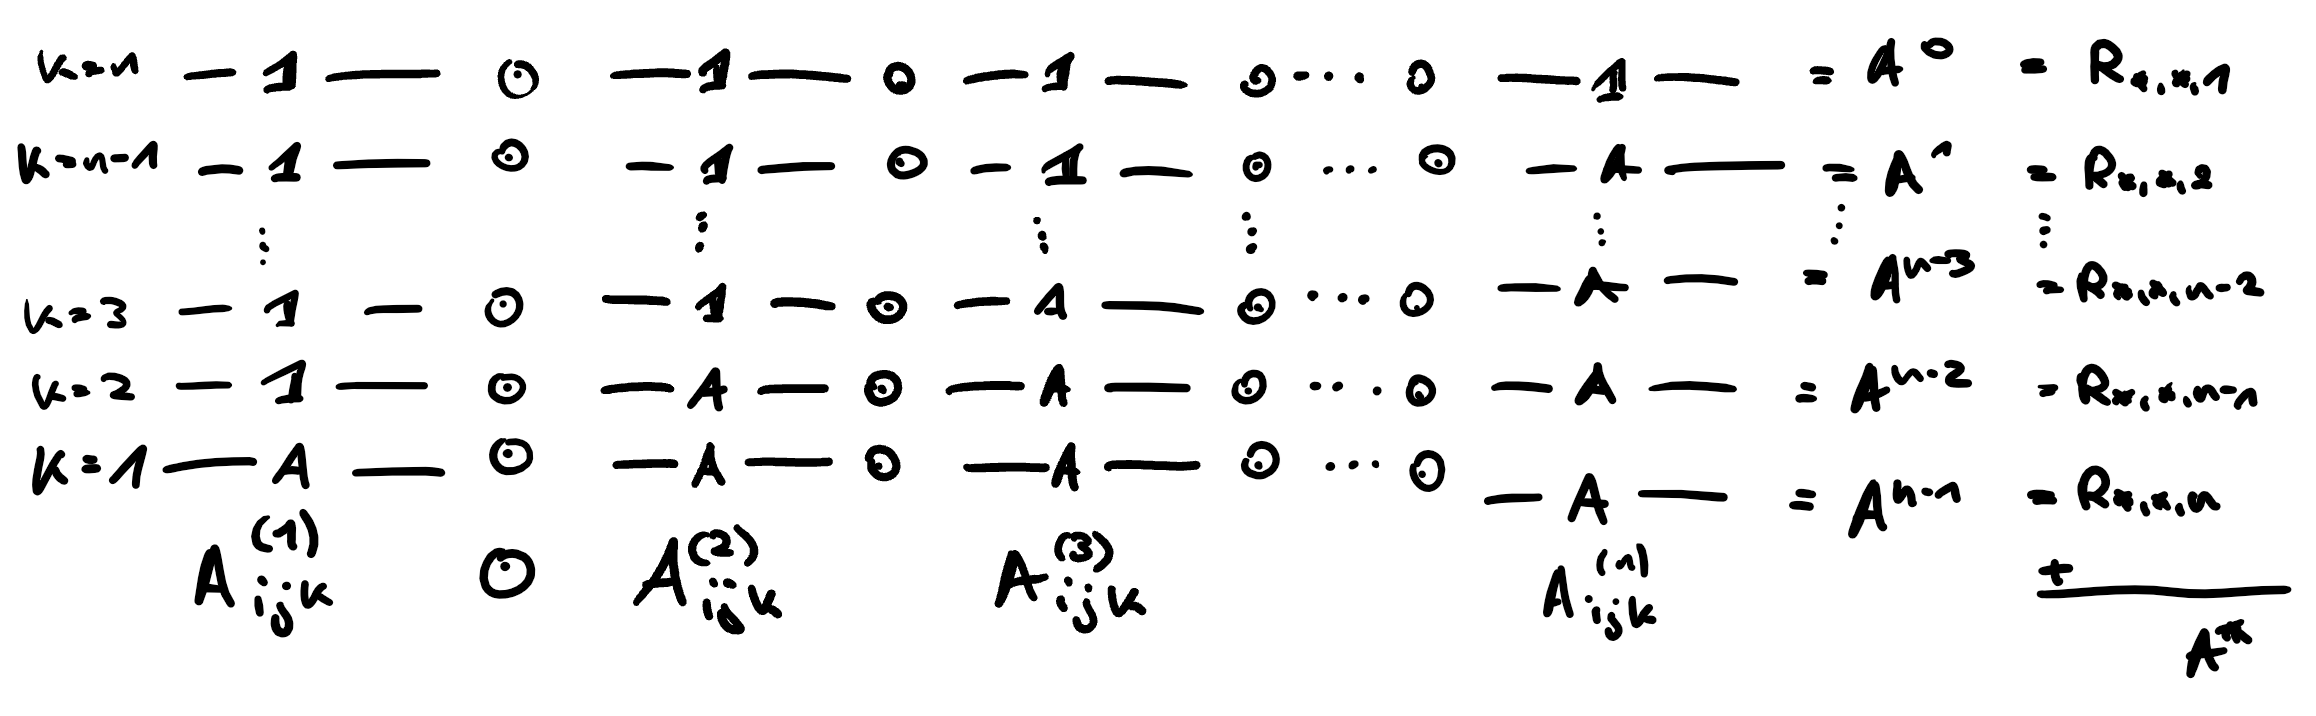
\includegraphics[width=\linewidth]{shortest_path_tensor.png}
    \caption{Visualized the shortest path tensors}
    \label{fig:shortest_path_tensor}
\end{figure}

The resulting expression comes out to be
$$A^*_{ij} = \sum_{k, t_1, \dots, t_{n-1} \in [n]} A^{(1)}_{it_1k}A^{(2)}_{t_1t_2k}A^{(3)}_{t_2t_3k}\dots A^{(n-1)}_{t_{n-2}t_{n-1}k}A^{(n)}_{t_{n-1}jk}$$
Which correspond to the Einsum string
$$it_1k, t_1t_2k, t_2t_3k, \cdots, t_{n-2}t_{n-1}k, t_{n-1}jk \to ij$$

\subsubsection{Receiving the paths}
To keep track of the paths we need to adapt the semiring. 
\begin{lemma}
    Let $V$ be a set then $(S := \R \times \powerset(\powerset(V)) \cup \{(\infty, \emptyset)\}, \oplus, \odot, (\infty, \emptyset), (0, \{\emptyset\}))$ is a semiring with the following operations:
    \begin{align*}
        (x_1, p_1) \oplus (x_2, p_2) &:= \begin{cases}
            (x_1, p_1) &\textrm{if}\quad x_1 < x_2 \\
            (x_2, p_2) &\textrm{if}\quad x_1 > x_2\\
            (x_1, p_1 \cup p_2) &\textrm{if}\quad x_1 = x_2
        \end{cases}\\
        (x_1, p_1) \odot (x_2, p_2) &:= (x_1 + x_2, \{s_1 \cup s_2 \mid s_1 \in p_1, s_2 \in p_2\}) =: (x_1 + x_2, p_1 \circ p_2)
    \end{align*}
\end{lemma}
\begin{proof}
    Because $\forall a \in \R\colon a < \infty$, $(\infty, 0)$ is indeed the neutral element of $\oplus$. The neutrality of $(0, \{\emptyset\})$ arises from the fact that $\forall (x, p) \in S\colon (x, p) \odot (0, \{\emptyset\}) = (x + 0, p \circ \{\emptyset\}) = (x, p)$. $(\infty, \emptyset)$ absorbs over $\odot$, because $\forall (x, p) \in S\colon (x, p) \odot (\infty, \emptyset) = (x + \infty, p \circ \emptyset) = (\infty, \emptyset)$. Commutivity and associativity of both $\oplus$ and $\odot$ result from the communativity and associativity of $+$, $\cup$ and $\circ$. If a $\infty$ is involved, these properties as well es distributivity also hold. Because $\odot$ is communative we only need to check left transitivity for when no $\infty$ is involved, namely 
    $$(x_1, p_1) \odot ((x_2, p_2) \oplus (x_3, p_3)) = ((x_1, p_1) \odot (x_2, p_2)) \oplus ((x_1, p_1) \odot (x_3, p_3))$$
    If $x_2 \neq x_3$ this is easy to see. Let w.l.o.g. $x_2 < x_3$ than we get
    \begin{align*}
        (x_1, p_1) \odot ((x_2, p_2) \oplus (x_3, p_3)) &= (x_1, p_1) \odot (x_2, p_2) = (x_1 + x_2, p_1 \circ p_2)\\
        ((x_1, p_1) \odot (x_2, p_2)) \oplus ((x_1, p_1) \odot (x_3, p_3)) &= (x_1 + x_2, p_1 \circ p_2) \oplus (x_1 + x_3, p_1 \circ p_3) = (x_1 + x_2, p_1 \circ p_2)
    \end{align*}
    Let us now consider the case $x_2 = x_3$.
    \begin{align*}
        (x_1, p_1) \odot ((x_2, p_2) \oplus (x_3, p_3)) &= (x_1, p_1) \odot (x_2, p_2 \cup p_3) = (x_1 + x_2, p_1 \circ (p_2 \cup p_3))\\
        ((x_1, p_1) \odot (x_2, p_2)) \oplus ((x_1, p_1) \odot (x_3, p_3)) &= (x_1 + x_2, p_1 \circ p_2) \oplus (x_1 + x_3, p_1 \circ p_3)\\ 
        &= (x_1 + x_2, (p_1 \circ p_2) \cup (p_1 \circ p_3))
    \end{align*}
    Thus, it is left to check whether $p_1 \circ (p_2 \cup p_3) \stackrel{?}{=} (p_1 \circ p_2) \cup (p_1 \circ p_3)$, in other words whether $\circ$ distributes over $\cup$.
    \begin{align*}
        x \in p_1 \circ (p_2 \cup p_3) &\Leftrightarrow \exists s_1 \in p_1, x' \in p_2 \cup p_3\colon x = s_1 \cup x'\\
        &\Leftrightarrow \exists s_1\in p_1, s_2 \in p_2, s_3 \in p_3 \colon x = s_1 \cup s_2 \cup s_3\\
        &\Leftrightarrow \exists s_1\in p_1, s_2 \in p_2, s_3 \in p_3 \colon x = (s_1 \cup s_2) \cup (s_1 \cup s_3)\\
        &\Leftrightarrow \exists x' \in p_1 \cup p_2, x'' \in p_1 \cup p_3 \colon x = x' \cup x''\\
        &\Leftrightarrow x \in (p_1 \circ p_2) \cup (p_1 \circ p_3)
    \end{align*}

    Closure is still to be checked and is not trivial, because all $(x, p)$ where $p \neq \emptyset$ are not in $S$. Let $(x_1, p_1), (x_2, p_2) \in S$. First assume $(x_1, p_1) \oplus (x_2, p_2) =: (x_3, p_3) \notin S$. The result must be in the form $x_3 = \infty, p_3 \neq \emptyset$. Thus, $x_1 = x_2 = \infty \Rightarrow p_1 = p_2 = \emptyset \Rightarrow p_3 = p_1 \cup p_2 = \emptyset$, which yields a contradiction.

    Let similarly assume $(x_1, p_1) \odot (x_2, p_2) =: (x_3, p_3) \notin S$. Again, it must hold that $x_3 = \infty, p_3 \neq \emptyset$. But $x_3 = \infty \Rightarrow x_1 = \infty \lor x_2 = \infty$. Let w.l.o.g $x_1 = \infty \Rightarrow p_1 = \emptyset$. $p_3 = p_1 \circ p_2 = \emptyset$, again a contraciction. Thus, $S$ is closed under $\oplus$ and $\odot$.
\end{proof}
Equipped with this semiring we can keep track of the paths. Let $V$ in the semiring be the set of edges. We build the adjacency matrix $A$ as follows:
$$A_{ij} = \begin{cases}
    (w(v_i, v_j), \{\{(v_i, v_j)\}\}) &\textrm{if}\quad i \neq j \land (v_i, v_j) \in V\\
    \infty &\textrm{if}\quad i \neq j \land (v_i, v_j) \notin V\\
    (0, \{\emptyset\}) &\textrm{if}\quad i = j
\end{cases}$$
Now $A^k_{ij}$ holds in the first component the weight of the shortest path between $v_i$ and $v_j$ with exactly $k$ edges and the second component holds all the paths. Here a path is represented by the set of its edges. As a shortest path will never pass an edge twice, this representation is sufficiant. 

\subsection{All pairs longest path}
The computation is exactly the same as in the All pairs shortest path problem. The only difference is the semiring in use. Here we need $(\R \cup \{-\infty\}, \max, +)$ and there must not exist a positive cycle. Then just compute $A^*$ and the entry $A^*_{ij}$ holds the longest path from $v_i$ to $v_j$. [Small note on convergency of $A^*$]

\subsection{Minimum weight spanning tree}
Here we need the observation that the edge $(v, u)$ is not included in the MST iff its weight is larger than the maximum weight of any path between $v$ and $u$. [Add proof] This we can model, by defining the weight of a path as the maximum of the weights of its edges. Then we compute the all pairs shortest path problem, but now we have exchanged the $+$-operation by the $\max$-operation, which means we have to use the $(\R \cup\{\infty\}, \min, \max)$ semiring. After computing $A^*$ we include the edge $(v_i, v_j)$ in the minimum weight spanning tree iff $A_{ij} \leq A^*_{ij}$.
[Diskuss conergency of $A^*$]

\subsection{Further Problems}
\begin{itemize}
    \item Marko Chaines. Using the semiring $([0, 1], +, \cdot)$ $A^k_{ij}$ holds the propability that an agent reaches $v_j$ starting at $v_i$ after $k$ steps if the weights of the edges symbolze the properbility that an agent moves along this edge.
    \item Reachability / Transitive hull. In an undirected unweighted graph, we ask the question whether a vertex $v_j$ is reachable starting at vertex $v_i$. For that we could just compute the shortest path and see whether $A^*_{ij}$ is infinite or not. But we can achieve the same with less information by just using the $(\{0, 1\}, \lor, \land)$ semiring and check whether $A^*_{ij} = 1$.
\end{itemize}


\section{Tropic polynomials}
Let $c_{e_1, \dots, e_m}(p)$ be the coefficiant in $p \in S[q_1, \dots q_m]$ of the monomial $p_1^{e_1}\dots p_m^{e_m}$. 

\begin{lemma}
    \label{lemma:prem_trop_poly}
    Let $A \in \N^{m \times n}$ and $w \in \R^n$. Let
    $$f := \bigoplus_{i=1}^{n} \sprod{w}{\hat e_i}\odot  q_1^{(A\hat e_i)_1}\dots q_m^{(A\hat e_i)_m} \in \T[q_1, \dots, q_m]$$
    be a tropic polynomial. Then it will hold that for all $l \in \N$
    $$c_{e_1, \dots, e_m}(f^{\odot l}) = \min\left\{\sprod{w}{v} \mid v \in \N^n, \sum_{i=0}^{n}v_i = l, Av=\smat{e_1\\\vdots\\e_m}\right\}$$
    Where $\min\emptyset:=\infty$.
\end{lemma}

\begin{proof}
    We will prove it by induction over $l$.
    \begin{itemize}
        \item[$l=0$:] $f^{\odot0} = 0$. There exists only one vector in $v \in \N^n$ such that $\sum_{i=0}^{n}v_i = 0$, which is the zero vector $\vec 0$. It is also clear that $\sprod{w}{\vec 0}= 0$ and $A\vec0=0$. So
        $$
            \min\left\{\sprod{w}{v} \mid v \in \N^n, \sum_{i=0}^{n}v_i = 0, Av=\smat{e_1\\\vdots\\e_m}\right\} = \begin{cases}
                0 &\textrm{if}\quad e_1, \dots, e_m = 0\\
                \infty &\textrm{else}
            \end{cases}
            \stackrel{\checkmark}{=}c_{e_1, \dots, e_m}(0)
        $$
        \item[$l=1$:] Because $\hat e_1, \dots, \hat e_n$ are all the vectors in $\N^n$, such that their components add up to 1, the equality is true by construction.
        \item[$l>1$:] Let $e := (e_1, \dots, e_m)^\top \in \N^m$
        \begin{align*}
            c_{e_1, \dots, e_m}(f^{\odot l}) &= c_{e_1, \dots, e_m}(f^{\odot (l-1)}\odot f) = \bigoplus_{\substack{f, g \in \N^m\\f+g=e}} c_{f_1, \dots, f_m}(f^{\odot (l-1)}) \odot c_{g_1, \dots, g_m}(f)\\
            &= \bigoplus_{\substack{f, g \in \N^m\\f+g=e}} \left(\bigoplus_{\substack{x \in \N^n\\\sum_{i=1}^{n}x_i = l-1\\Ax=f}}\sprod{w}{x}\right) \odot \left(\bigoplus_{\substack{y \in \N^n\\\sum_{i=1}^{n}y_i = 1\\Ay=g}}\sprod{w}{y}\right)\\
            &= \bigoplus_{\substack{f, g \in \N^m\\f+g=e}}\bigoplus_{\substack{x, y \in \N^n\\\sum_{i=1}^{n}x_i = l-1\\\sum_{i=1}^{n}y_i = 1\\Ax=f, Ay=g}} \underbrace{\sprod{w}{x} \odot \sprod{x}{y}}_{\sprod{w}{x+y} =: \sprod{x}{v}} = \bigoplus_{\substack{f, g \in \N^m\\f+g=e}}\bigoplus_{\substack{v \in \N^n\\\sum_{i=1}^{n}v = l\\Av=f+g=e}} \sprod{w}{v}\\
            &= \bigoplus_{\substack{v \in \N^n\\\sum_{i=1}^{n}v = l\\Av=e}} \sprod{w}{v} = \min\left\{\sprod{w}{v} \mid v \in \N^n, \sum_{i=0}^{n}v_i = l, Av=e\right\}
        \end{align*} 
    \end{itemize}
\end{proof}

\begin{theorem}
    Let $\min \stackrel{!}{=} w^\top x$ s.t. $Ax=b$ an ILP, such that all columns of $A$ sum up to the same number $\alpha \in \N^*$. We wat the ILP, to have solutions, so $k = \frac{1}{\alpha}\sum_{i=1}^{m}b_i \in \N$ exists. Let $f \in \T[q_1, \dots, q_m]$ be like in Lemma \ref{lemma:prem_trop_poly}, so 
    $$f := \bigoplus_{i=1}^{n} \sprod{w}{\hat e_i}\odot  q_1^{(A\hat e_i)_1}\dots q_m^{(A\hat e_i)_m}$$
    Then $c_{b_1, \dots, b_m}(f^{\odot k})$ solves the ILP 
\end{theorem}

\begin{proof}
    Because of Lemma \ref{lemma:ilp_pre1}, for all solutions $x \in \N^n$ of $Ax=b$ will hold that $\sum_{i=1}^{n}x_i = k$. No it is just a matter of rewriting the solution of the ILP and applying Lemma \ref{lemma:prem_trop_poly}.
    \begin{align*}
        \min\{\sprod{w}{x} \mid x \in \N^n, Ax=b\} &\stackrel{\ref{lemma:ilp_pre1}}{=} \min\left\{\sprod{w}{x} \mid x \in \N^n, \sum_{i=1}^{n}x_i = k , Ax=b\right\}\\
        &\stackrel{\ref{lemma:prem_trop_poly}}{=} c_{b_1, \dots, b_m}(f^{\odot k})
    \end{align*}
\end{proof}

\section{Old and wrong solution}
\subsection{Final writeup}
Now we need to find a $\vec\mu$ that minizes $k(\vec\mu)$. I will present the algorithm to find this $\vec\mu$ up front and then show that the result is actually correct. First we need to define an operation. 
\begin{definition}
    Let $M \in \N^{m\times n}$ be a matrix. Then $\Delta(M) \in \Z^{(n-1)\times m}$ is also a matrix such that 
    $$\Delta(M)_{i,j} = M_{j,i} - M_{j,i+1}$$
\end{definition}

\begin{algorithm}
    \label{_algo}
    \textbf{Input: } $A\in\N^{m\times n} \neq 0, \vec b \in \N^m$. Let $\vec a_1, \dots, a_n\in\N^m$ be the columns of $A$.\\
    \textbf{Output: } $\vec\mu\in\R^m$ that minimizes the function:
    $$k(\vec\mu) = \frac{\sprod{\vec\mu}{\vec b}}{\min_{j\in[n]}\sprod{\vec\mu}{\vec a_j}}$$
    Steps:
    \begin{enumerate}
        \item Sort all columns in $A$ by their column sum - $O(n \log n + m \cdot n)$
        \item Perform the choice of basis algorithm, to select a basis of the column space of $A$. Let the basis be $[\vec a_{j_1}, \dots, \vec a_{j_r}]$. Create a new matrix $A' := (\vec a_{j_1}, \dots, \vec a_{j_r}) \in \N^{m \times r}$ - $O(m^2 \cdot n)$
        \item Calculate $\Delta(A')$ and then a basis of $\solspace(\Delta(A'), \vec0)$ - $O(n^2 \cdot m)$
        \item Calculate a basis of $\solspace(A^\top, \vec0)$ - $O(n^2 \cdot m)$
        \item Find a $\vec\mu \in \solspace(\Delta(A'), \vec0) \setminus \solspace(A^\top, \vec0)$. For example write basis vectors of solution space of 4. on the left and basis vectors of solution space of 5. on the right in a matrix. Do basis selection. There will be a base vector selected from the right. This can be $\vec\mu$. - $O(m^3)$
    \end{enumerate}
    This yields a runtime of $O(n \cdot m^2 + n^2 \cdot m + m^3) = O(n^2 \cdot m + m^3)$.
\end{algorithm}

Now we have to answer the question of correctness. And we will do that in a few steps.
\begin{enumerate}
    \item Make sure, that the $\vec\mu$ actaully exists, meaning: $\solspace(\Delta(A'), \vec0) \setminus \solspace(A^\top, \vec0) \neq \emptyset$.
    \item Make sure, that the $\vec\mu$ is actaully in the domain of $k$, meaning $\vec\mu \in U \Leftrightarrow \forall j \in [n]\colon \sprod{\vec a_j}{\vec\mu}>0$.
    \item Make sure, that the $\mu$ minimizes $k(\vec\mu)$.
\end{enumerate}
First define some notions, that we will need throughout:
\begin{definition}
    \label{def:_algo_basic}
    Let $A \in \N^{m \times n}$ be a matrix, such that $A$ does not contain a zero column. Let $\vec a_j$ be the $j$-th column of $A$. Let $B := [\vec a_{j_1}, \dots, \vec a_{j_r}]$ and $A' \in \N^{m\times r}$ be as in step 2 in the algorithm \ref{algo}. Let $\vec b \in \N^m$. Let $U := \{\vec\mu \in \R^m\mid \forall j \in [n]\colon\sprod{\vec\mu}{\vec a_j} > 0\}$. Let $U_j := \{\vec\mu \in U \mid \forall j'\in[n]\colon \sprod{\vec\mu}{\vec a_j} \leq \sprod{\vec\mu}{\vec a_{j'}}\}$. Let $k\colon \N^m\to\R$ be defined as 
    $$k(\vec\mu) := \frac{\sprod{\vec\mu}{\vec b}}{\min_{j\in[n]}\sprod{\vec\mu}{\vec a_j}}$$
\end{definition}

\subsubsection{Existance of a result}
\begin{lemma}
    Let $A, A'$ be as in definition \ref{def:algo_basic}. Then $\dim(\solspace(\Delta(A'), \vec0)) > \dim(\solspace(A^\top, \vec0))$.
\end{lemma}
\begin{proof}
    Observe that $\dim(\solspace(\Delta(A'), \vec0)) = \nullity(\Delta(A'))$ and $\dim(\solspace(A, \vec0)) = \nullity(A)$. By construction: $\rank(A) = \rank(A^\top) = \rank(A') = r$. As $\Delta(A')$ has only $r-1$ rows, $\rank(\Delta(A')) \leq r-1 < r$. Now we can apply the Rank-nullity theorem to $A^\top$ and $\Delta(A')$.
    $$m = \rank(A^\top) + \nullity(A^\top) \Leftrightarrow \nullity(A^\top) = m - r$$
    $$m = \rank(\Delta(A')) + \nullity(\Delta(A')) < r + \nullity(\Delta(A'))\Leftrightarrow \nullity(\Delta(A')) > m - r$$
    Combining these two results yields $\nullity(\Delta(A')) > \nullity(A^\top)$ the result we wanted to show.
\end{proof}
The difference of 2 vector spaces, of which the first one has a bigger dimesnion, yields always a nonempty set of vectors. Thus indeed $\solspace(\Delta(A'), \vec0) \setminus \solspace(A^\top, \vec0) \neq \emptyset$. But not only that, it also ensures that the method of selecting a $\vec\mu \in \solspace(\Delta(A'), \vec0) \setminus \solspace(A^\top, \vec0)$ proposed in step 5 does yield a solution.

\subsubsection{Is the result of the algorithm a possible solution}
In this section we will show that $\vec\mu \in U \Leftrightarrow \forall j \in [n]\colon \sprod{\vec a_j}{\vec\mu}>0$. We know that by construction $\vec\mu \notin \solspace(A^\top, \vec0)$ which translates to $\forall j \in [n]\colon\sprod{\vec\mu}{\vec a_j} \neq 0$. Furthermore because $\vec\mu\in\solspace(\Delta(A'), \vec0)$ we know that $\sprod{a_{j'_1}}{\vec\mu} = \dots = \sprod{a_{j_r}}{\vec\mu} =: d$. We know that $d \neq 0$ and we can thus w.l.o.g. assume that $d>0$, because if $d$ would be negative, we could replace $\vec\mu$ by $-\vec\mu$ which would yield a positive $d$. It is left to show that the dot-product with all other columns of $A$ is also positive:

\begin{lemma}
    \label{lemma:non_basis_vecs_greater}
    Let $A$ and $[\vec a_{j_1}, \dots, \vec a_{j_r}]$ as in definition \ref{def:algo_basic}. Let $\vec a_l$ be any column of $A$, that did not get selected by the basis selection. Let $\vec\mu \in \R^m$ be a result from algorithm \ref{algo}, thus $\sprod{\vec a_{j_1}}{\vec\mu} = \dots = \sprod{\vec a_{j_r}}{\vec\mu} =: d > 0$. Then it will hold, that 
    $$\sprod{\vec a_l}{\vec\mu} \geq d$$
\end{lemma}
\begin{proof}
    As $\vec a_l$ was not selected as a basis, we know that it linearly dependend on the columns on its left in the matrix $A$, where the columns have been sorted by their column sum in an ascending order.  Let the set of basis vectors that are on the left of $\vec a_l$ be $\{\vec a_{j_1}, \dots, \vec a_{j_s}\}$. Thus we know that their column sum is never larger than the column sum of $\vec a_l$. In other words:
    $$\forall k \in [s]\colon\sum_{i=1}^{m} \left(\vec a_{j_k}\right)_i \leq \sum_{i=1}^{m} \left(\vec a_l\right)_i$$
    Because $\vec a_{j_l}$ is linearly dependend on those previous columns and the vectors $\vec a_{j_1}, \dots, \vec a_{j_s}$ are a basis of that space, we know that there must exist $\lambda_1, \dots, \lambda_s$ such that:
    $$\sum_{k=1}^{s}\lambda_k \vec a_{j_k} = \vec a_l$$
    Now we will consider the component sum of $\vec a_l$
    \begin{align*}
        \sum_{i=1}^{m} (\vec a_l)_i &= \sum_{i=1}^{m} \left(\sum_{k=1}^{s}\lambda_k \vec a_{j_k}\right)_i = \sum_{i=1}^{m} \sum_{k=1}^{s}\lambda_k \left(\vec a_{j_k}\right)_i = \sum_{k=1}^{s} \lambda_k \cdot\underbrace{\sum_{i=1}^{m} \left(\vec a_{j_k}\right)_i}_{\leq \sum_{i=1}^{m} (\vec a_l)_i}\\
        &\leq \sum_{k=1}^{s} \lambda_k \cdot\sum_{i=1}^{m} (\vec a_l)_i = \left(\sum_{k=1}^{s} \lambda_k\right) \cdot\left(\sum_{i=1}^{m} (\vec a_l)_i\right)\\
        \Rightarrow\quad 1 &\leq \sum_{k=1}^{s} \lambda_k
    \end{align*}
    With this result we are ready to compute the dot product.
    $$\sprod{\vec a_{l}}{\vec\mu} = \largesprod{\sum_{k=1}^{s}\lambda_k \vec a_{j_k}}{\vec\mu} = \sum_{k=1}^{s}\lambda_k \underbrace{\sprod{\vec a_{j_k}}{\vec\mu}}_d = d\cdot \underbrace{\sum_{k=1}^{s}\lambda_k}_{\geq 1} \geq d$$
\end{proof}
Now we know that for all columns of $A$, namely $\vec a_j$ it will hold that:
$$\sprod{\vec a_j}{\vec\mu} \geq d > 0$$

\subsubsection{Correctness of the solution}
Before we discuss whether we can indeed find the minimum, we determine what $k(\vec\mu)$ actually is, where $\vec\mu$ is the result of our algorithm. For that, we can still benefit from lemma \ref{lemma:non_basis_vecs_greater}. It says, that $\sprod{\vec a_{j_i}}{\vec\mu} = d$ is actually the smallest possible dot-product. Thus
$$k(\vec\mu) = \frac{1}{d}\cdot\sprod{\vec\mu}{\vec b}$$
Now we will see, that this is actually the smallest possible value. To see that remember that $k(\vec\mu)$ is piecewise strictly monotone or constant. It is apparent that the minimumn can only be reached in a montone region. Remember that (INSERT REF) $\restrict{k}{U_{j_1} \cap \dots \cap U_{j_r}}$ is constant iff $\vec b \in \Span(\vec a_{j_1}, \dots, a_{j_r})$. Thus we have to only consider all different basis of the column space in $A$. So if $[\vec a_{j'_1}, \dots, \vec a_{j'_r}]$ is a different basis from $[\vec a_{j_1}, \dots, \vec a_{j_r}]$, we need to show that $k(\vec\mu') \geq k(\vec\mu)$ for $\vec\mu \in U_{j_1} \cap \dots \cap U_{j_r}$ and $\vec\mu' \in U_{j'_1} \cap \dots \cap U_{j'_r}$. And this will be done by the next lemma:

\begin{lemma}
    Let $A$ and $B := [\vec a_{j_1}, \dots, \vec a_{j_r}]$ as in definition \ref{def:algo_basic} and let the columns of $A$ be sorted by their column sum in an ascending order. Let $B' := [\vec a_{j'_1}, \dots, \vec a_{j'_r}]$ be a different basis, also such that the vectors are sorted based on their column sum ascendingly. Let $\vec\mu \in U_{j_1} \cap \dots \cap U_{j_r}$ and $\vec\mu' \in U_{j'_1} \cap \dots \cap U_{j'_r}$, thus $\sprod{\vec a_{j_1}}{\vec\mu} = \dots = \sprod{\vec a_{j_r}}{\vec\mu} =: d > 0$ and $\sprod{\vec a_{j'_1}}{\vec\mu'} = \dots = \sprod{\vec a_{j'_r}}{\vec\mu'} =: d' > 0$. Then $k(\vec\mu) = k(\vec\mu')$.
\end{lemma}
\begin{proof}
    We will show that not only $\sprod{\vec a_{j'_1}}{\vec\mu'} = \dots = \sprod{\vec a_{j'_r}}{\vec\mu'} = d'$ but this also holds for $B$, namely $\sprod{\vec a_{j_1}}{\vec\mu'} = \dots = \sprod{\vec a_{j_r}}{\vec\mu'} = d'$. From this, is it clear that $\vec\mu' \in U_{j_1} \cap \dots U{j_r}$ and because $\restrict{k}{U_{j_1} \cap \dots U{j_r}}$ is constant and also $\vec\mu \in U_{j_1} \cap \dots U{j_r}$, we can conclude that $k(\vec\mu) = k(\vec\mu')$. So in the following we will show that indeed $\sprod{\vec a_{j_1}}{\vec\mu'} = \dots = \sprod{\vec a_{j_r}}{\vec\mu'} = d'$. This we will do in 3 steps:
    \begin{enumerate}
        \item The coordnates of any basis vector in $B'$ expressed in terms of $B$ sum up to 1.
        \item The coordnates of any basis vector in $B$ expressed in terms of $B'$ sum up to 1.
        \item Conclude that $\sprod{\vec a_{j_k}}{\vec\mu'} = d'$ for all $k \in [r]$
    \end{enumerate}

    Let $\vec a_{j'_l}$ be an arbetrairy vector of $B'$. Obviously there exists a unique linear combination of the vectors $B$:
    $$\vec a_{j'_l} = \sum_{k=1}^{r}\lambda_k\vec a_{j_k}$$
    If $\vec a_{j'_l}$ is also in $B$, meaning that there exists a $s$ such that $\vec a_{j'_l} = \vec a_{j_s}$, that it will hold that $\lambda_s = 1$ and all other $\lambda_k$'s are zero. Thus
    $$\sum_{k=1}^{r}\lambda_k = 1$$

    Now we have to consider the case where $\vec a_{j'_l}$ is not part of $B$. As $\vec a_{j'_l}$ has not been selected in the choice of basis algorithm, it must be a linear combination of the basis vectors in $B$ that stand left in the sorted matrix $A$. Thus:
    $$\vec a_{j'_l} = \sum_{k=1}^{s}\lambda_k\vec a_{j_k} \qquad\textrm{with}\quad \forall k \leq s\colon\sum_{i=1}^{m}(\vec a_{j_k})_i \leq \sum_{i=1}^{m}(\vec a_{j'_l})_i$$
    This result yields us following when considering the column sum of $\vec a_{j'_l}$:
    \begin{align*}
        \sum_{i=1}^{m} (\vec a_{j'_l})_i &= \sum_{i=1}^{m} \left(\sum_{k=1}^{s}\lambda_k \vec a_{j_k}\right)_i = \sum_{i=1}^{m} \sum_{k=1}^{s}\lambda_k \left(\vec a_{j_k}\right)_i = \sum_{k=1}^{s} \lambda_k \cdot\underbrace{\sum_{i=1}^{m} \left(\vec a_{j_k}\right)_i}_{\leq \sum_{i=1}^{m} (\vec a_{j'_l})_i}\\
        &\leq \sum_{k=1}^{s} \lambda_k \cdot\sum_{i=1}^{m} (\vec a_{j'_l})_i = \left(\sum_{k=1}^{s} \lambda_k\right) \cdot\left(\sum_{i=1}^{m} (\vec a_{j'_l})_i\right)\\
        \Rightarrow\quad 1 &\leq \sum_{k=1}^{s} \lambda_k = \sum_{k=1}^{r} \lambda_k
    \end{align*}
    The last step - replacing $r$ with $s$ - just corresponds with the fact, that the linear combination of the basis vectors is unique. And as we have found one, that only include the first $s$ basis vectors, we know that $\lambda_{s+1} = \dots = \lambda_r = 0$

    Now remind yourself that, it must hold that $\vec\mu' \in U_{j'_1} \cap \dots \cap U_{j'_r}$ by assumption. This only happens, if $\sprod{\vec a_{j'_l}}{\vec\mu'} = d'$ gives the smallest dot-product. So all other dot-products are actually bigger. This we can also use:
    $$d' = \sprod{\vec a_{j'_l}}{\vec\mu'} = \sum_{k=1}^{s}\lambda_k\underbrace{\sprod{\vec a_{j_k}}{\vec\mu'}}_{\geq d'} \geq d'\cdot \sum_{k=1}^{s}\lambda_k \quad\Rightarrow 1 \geq \sum_{k=1}^{s}\lambda_k = \sum_{k=1}^{r}\lambda_k$$
    Combining these two results yields again
    $$\sum_{k=1}^{r}\lambda_k = 1$$
    This concludes the first step of our proof. Onto the second:

    The second step involves some change of basis. We have seen that the coordinates of the basis vectors in $B'$ based on $B$ add up to 1. Let $T$ be the change of basis matrix from $B'$ to $B$. The abovementioned property can be reframed, as that the column sum of every colum in $T$ is equal to 1. Or in other words that $\opvec(1)^\top T = \opvec(1)^\top$. This property also holds for its inverse, because of this:
    $$\opvec(1)^\top T = \opvec(1)^\top \Leftrightarrow \opvec(1)^\top T\cdot T^{-1} = \opvec(1)^\top\cdot T^{-1} \Leftrightarrow \opvec(1)^\top = \opvec(1)^\top\cdot T^{-1}$$
    Thus if you express a basis vector from $B$ in coordinates of $B'$, the component sums ends up to be 1 as well. Let $\vec a_{j_l}$ be an arbetrairy vector from the first basis. We thus know that
    $$\vec a_{j_l} = \sum_{k=1}^{r}\lambda'_k \vec a_{j'_k} \qquad \textrm{with}\quad \sum_{k=1}^{r}\lambda'_k = 1$$
    This concludes the second step in the proof. The last step is very short:
    $$\sprod{\vec a_{j_l}}{\vec\mu'} = \largesprod{\sum_{k=1}^{r}\lambda'_k \vec a_{j'_k}}{\vec\mu'} = \sum_{k=1}^{r} \lambda'_k \underbrace{\sprod{\vec a_{j'_k}}{\vec\mu'}}_{=d'} = d' \cdot \underbrace{\sum_{k=1}^{r} \lambda'_k}_{=1} = d'$$
\end{proof}

\subsection{Discussion on slack variables}
Normally, an ILP is not given as a system of equations $A\vec x = \vec b$, where all entries in $\vec x$ are natural numbers, but a system of inequalities $A\vec x \leq \vec b$, where all entries in $\vec x$ are whole numbers. This notation does not make immediate sense, as it seams like we are comparing two vectors with a $\leq$-sign. What is ment is, that for each component of $A\vec x$ must be smaller or equal the the corresponding component in $\vec b$. 

To convert from the the $\leq$-version to the $=$-version, you introduce another variable vector $\vec s$, resulting in linear system of equations:
$$A\vec x + \vec s = \vec b \qquad \vec x \in \N^n, \vec s \in\N^m$$
The variables in $\vec s$ are called slack variables. But instead of changing the equation we are dealing with, we can also just modify $A$ and $\vec x$ to get to the same result. If you just attach the vector $\vec s$ onto $\vec x$: $\vec x \mapsto (x_1, \dots, x_n, s_1, \dots, s_m)^\top \in \N^{n+m}$ and attach an identity matrix into $A$: $A \mapsto (A \mid\imat_m) \in \N^{m \times (n + m)}$. Thus, if we construct $A$ using the common method of slack variables, the columns of $A$ will include all possible unit vectors.

This fact hugely impacts the results we can expect from the algorithm. Let us think it through: When sorting the columns of $A$ by their column sum, all of these columns will be sorted to the beginning, as they have the minimal column sum of $1$. Because we have all standart basis vectors in the front of $A$, they will all be selected by the choice of basis algorithm. Thus $A'$ will be some column permutation of the identity matrix. You can easily check that $\Delta(A')\opvec(1) = \vec 0$ and because all column sum in $A$ are postive, this means that $A^\top \opvec(1) > \vec 0$. Thus the algorithm could pick $\vec\mu = \opvec(1)$.

Why is this an issues now? $\opvec(1)$ represents the matrix $A$ itself without alterations. And as the algorithm spits out the best possible matrizes, we cannot imporve $A$ even further. Which means, that of we use slack variables, the resulting matrix is not improvable.